\documentclass{article}
\usepackage[a4paper, total={6in, 8in}]{geometry}
\usepackage{graphicx}

\begin{document}
\graphicspath{{./}}
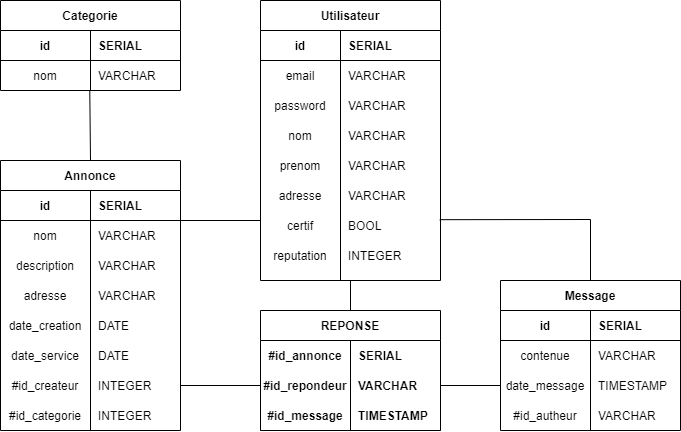
\includegraphics[width=8cm, height=15cm]{Schema-relationnel-BDD.png}\\\\
Serial est un type de donnée qui sert à créer des id, il est équivalent à dire que l'on auto-incremente les id à chaque INSERT.\\\\
\textbf{Utilisateur(\underline{id}, email, password, nom, prenom, adresse, certif, reputation)}\\\\
\textbf{Categorie(\underline{id}, nom)}\\\\
\textbf{Annonce(\underline{id}, nom, description, adresse, date\_creation, date\_service, \#id\_createur, \#id\_categorie)}\\
id\_createur clef étrangère de Utilisateur.\\
id\_categorie clef étrangère de Categorie.\\\\
\textbf{Message(\underline{id}, contenue, date\_message, \#id\_auteur)}\\
id\_auteur clef étrangère de Utilisateur.\\\\
\textbf{Reponse(\underline{\#id\_annonce, \#id\_repondeur, \#id\_message})}\\
id\_annonce clef étrangère de Annonce.\\
id\_repondeur clef étrangère de Utilisateur.\\
id\_message clef étrangère de Message.\\\\

Lorsqu'un utilisateur clique sur une annonce qu'il a crée, on lui affiche la liste de personne ayant répondu. Après son choix, il nous reste alors tout les messages entre le créateur de l'annonce et le repondeur.
\end{document}
